\documentclass[10pt,a4paper]{article}
\usepackage[latin1]{inputenc}
\usepackage[T1]{fontenc}
\usepackage{amsmath}
\usepackage{amsfonts}
\usepackage{amssymb}
\usepackage{hyperref} %links a archivos
\usepackage{graphicx} %cargar imagenes
\everymath{\displaystyle}

\author{Nellmeldin, Fernando}
\title{Mec�nica Computacional 2011 \\ Gu�a de Referencia}
\date{}
\begin{document}
\maketitle
\newpage
\tableofcontents
\newpage
\section{Ejercicio 1 - Difusi�n del Calor}
Los problemas de transferencia de calor expresan la satisfacci�n de la conservaci�n de
la energ�a en el campo de la f�sica. Una representaci�n de los mismos viene dada por el
siguiente problema matem�tico:
Hallar el campo de temperaturas T(x,y,z;t) tal que

\begin{align}
\begin{array}{l l}
\rho c \frac{\partial T}{\partial t} = \nabla \cdotp ( k \nabla T ) + G  - h (T - T_{amb}) & \quad \forall x \in \Omega \\[3mm]
\text{Sujeto a las siguientes condiciones} \\[2mm]
T = \bar{T} & \quad \forall x \in r_T \\[1mm]
q = -k \nabla T = \bar{q} & \quad \forall x \in r_q \\[1mm]
q = -k \nabla T + h (T - T_{ref}) & \quad \forall x \in r_h \\[1mm]
T = T^0 & \quad \forall x \in \omega \quad y \quad t = 0
\end{array}
\end{align}
$\rho$ = densidad; c = calor espec�fico; k = conductividad t�rmica; h = coeficiente de
convecci�n; G = fuente de calor; $T_{amb}$ = temperatura del medio ambiente.


\subsection{Parte A}
Considerar una simetr�a del problema tal que puede ser resuelto en 1D, L = 1,
$\rho$c = 1, k = 1, h = 0 y G = 0. Entonces el problema queda planteado como:

Hallar el campo de temperaturas T(x,t) tal que
\begin{align}
\frac{\partial T}{\partial t} = \frac{ \partial{^2 T}} {\partial{t^2}} \quad \forall x \in [0;1] \\[3mm]
\text{Sujeto a las siguientes condiciones} \notag\\[2mm]
T(0,t) = 1 \notag\\[1mm]
T(1,t) = 0 \\[1mm]
T(x,0) = 1 - x \notag
\end{align}

Se discretiza el tiempo con Forward Euler y la derivada segunda con m�todo de segundo orden:
\begin{align}
\frac{T_{i}^{n+1} - T_{i}^{n}} {\Delta t} = \frac{T_{i+1}^{n} - 2 T_{i}^{n} + T_{i-1}^{n}} {\Delta x^2} \notag\\
\Rightarrow T_{i}^{n+1} = T_{i}^{n} + \frac{\Delta t}{\Delta x^2} ( T_{i+1}^{n} - 2 T_{i}^{n} + T_{i-1}^{n} )
\end{align}

Se elige un paso $\Delta x$ de $1/3$. \\
Como la relaci�n: $ F_0 = \frac{ \Delta t }{ \Delta x^2 } $ debe cumplir $F_0 < 1/2 $ donde $F_0$ es el n�mero de Fourier, se elige un $\Delta t = 1/36$. \\

As�, se obtienen las siguientes condiciones iniciales:
Sea 
\begin{align}
	T_i^0 = 1 - x \Rightarrow 
				\left\{ 
						\begin{array}{l} 
							T_0^0 = 1 \\ 
							T_1^0 = 2/3 \\ 
							T_2^0 = 1/3 \\ 
							T_3^0 = 0 
						\end{array}
				\right.
\end{align}
El stencil tiene la siguiente forma final:
\begin{align} T_i^{n+1} = T_i^n + \frac{1}{4} \left( T_{i+1}^n - 2 T_{i}^n + T_{i-1}^n \right)\end{align}

El algoritmo \href{guiaRefEj1a.sci}{guiaRefEj1a.sci} resuelve este problema de manera iterativa.


\subsection{Parte B}
Resolver el problema en 1D, L = 1, $\rho$c = 1, k = 1, h = 1, $T_{amb}$ = 0, con 
\begin{align} G(x) = \left\{ 
			\begin{array}{l l} 
						1 & \forall x \leq 1/2 \\ 
						0 & \forall x    > 1/2 \\ 
		    \end{array} 
	  \right. 
\end{align}

Luego, el problema queda planteado como: \\
Hallar el campo de temperaturas T(x,t) tal que
\begin{align}
	\begin{array}{l l}
	\frac{\partial T}{\partial t} - \frac{\partial^2 T}{\partial x^2} + T = 1 	& \quad \forall x \in [0 , 1/2] \\[3mm]
	\frac{\partial T}{\partial t} - \frac{\partial^2 T}{\partial x^2} + T = 0 	& \quad \forall x \in ( 0,1/2]\\[3mm]
	\text{Sujeto a las condiciones de contorno} \\[3mm]
	T(0,t) = 1 \\[3mm]
	\frac{\partial T}{\partial x }(1,t) = 0 \\[3mm]
	T(x,0) = 1 - x \\
	\end{array}
\end{align}


Se discretiza el tiempo con Forward Euler y la derivada segunda con m�todo de segundo orden:
\begin{align}
\frac{T_{i}^{n+1} - T_{i}^{n}} {\Delta t} - \frac{T_{i+1}^{n} - 2 T_{i}^{n} + T_{i-1}^{n}} {\Delta x^2} + T_i^n = G_i \notag\\[2mm]
\Rightarrow T_{i}^{n+1} = \Delta t (G_i - T_{i}^{n} )  + \frac{\Delta t}{\Delta x^2} ( T_{i+1}^{n} - 2 T_{i}^{n} + T_{i-1}^{n} ) + T_i^n
\end{align}

Se elige un paso $\Delta x$ de $1/4$. \\

Como la relaci�n: $ F_0 = \frac{ \Delta t }{ \Delta x^2 } $ debe cumplir $F_0 < 1/2 $ donde $F_0$ es el n�mero de Fourier, se elige un $\Delta t = 1/64$. \\
As�, se obtienen las siguientes condiciones iniciales:
\begin{align}
	T_i^0 = 1 - x \Rightarrow 
				\left\{ 
						\begin{array}{l} 
							T_0^0 = 1 \\ 
							T_1^0 = 3/4 \\ 
							T_2^0 = 1/2 \\ 
							T_3^0 = 1/4 \\
							T_4^0 = 0 
						\end{array}
				\right.
\end{align}
De la condici�n de contorno tipo Neumann, se obtiene:
\begin{align}
\frac{\partial T}{\partial x} = \frac{T_{i+1}^{n} - T_{i-1}^{n}} {2 \Delta x}  = 0 \Rightarrow T_{i+1}^n = T_{i-1}^n \text{ en } x = 1
\end{align}

El stencil tiene la siguiente forma final:
\begin{align}
T_{i}^{n+1} = \frac{1}{64} (G_i - T_{i}^{n} )  + \frac{1}{4} ( T_{i+1}^{n} - 2 T_{i}^{n} + T_{i-1}^{n} ) + T_i^n
\end{align}

El algoritmo \href{guiaRefEj1b.sci}{guiaRefEj1b.sci} resuelve este problema de manera iterativa.





\subsection{Parte C}
Considerar el problema de transferencia de calor bidimensional, en presencia de
3 fuentes de calor distribuidas, con simetr�a con respecto al eje x, tal que puede
resolverse en una dimensi�n. Las dimensiones de la placa se muestran en la siguiente figura:

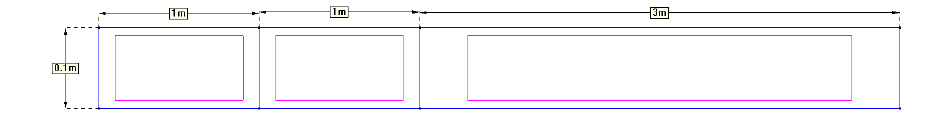
\includegraphics[width=\textwidth]{imgEj1c.png}
El problema puede ser planteado como:
\begin{align}
\begin{array}{l l}
	\frac{\partial^2 T}{\partial x^2} = - f(x) \\[3mm]
	\text{Sujeto a las siguientes condiciones de contorno:} \\[2mm]
	T(0) = 100 \\[3mm]
	\frac{\partial T}{\partial x}(5) = 0 
\end{array}
\end{align}

Donde
\begin{align}
 f(x) = \left\{ 
			\begin{array}{l l} 
						-10 & \forall \;x 	\in [0,1]\\ 
						5 	& \forall \;x    	\in (1,2] \\ 
						-1 	& \forall \;x   	\in (2,5] \\ 
		    \end{array} 
	  \right. 
\end{align}


Adem�s, se debe verificar la continuidad y derivabilidad en los extremos de cada uno de los intervalos interiores.

Se discretiza la derivada segunda con m�todo de segundo orden:
\begin{align}
\frac{T_{i+1} - 2 T_{i} + T_{i-1}} {\Delta x^2} = - f_i 
\Rightarrow T_{i+1} - 2 T_{i} + T_{i-1} = - f_i \Delta x^2
\end{align}

Utilizando la condici�n de Contorno tipo Dirichlet en $x = 0$ obtenemos el valor $$T_0 = 100$$
Asimismo, de la condici�n de contorno tipo Neumann, en $x = 5$ se obtiene:
\begin{align}
\frac{\partial T}{\partial x} = \frac{T_{i+1} - T_{i-1}} {2 \Delta x}  = 0 \Rightarrow T_{i+1} = T_{i-1} \text{ en } x = 5
\end{align}

El algoritmo \href{guiaRefEj1c.sci}{guiaRefEj1c.sci} resuelve este problema.

\newpage







\section{Ejercicio 4 - Flujo Potencial}
En un problema de flujo de flu�dos bidimensional, inv�scido, irrotacional e incompresible (flujo potencial), las componentes de velocidades $(u,v)$ en las direcciones $x$ e $y$, y el potencial de velocidad satisfacen las ecuaciones:
\begin{align}
\begin{array}{l l}
	u = \frac{\partial \phi }{\partial x} ; \\[4mm]
	v = \frac{\partial \phi }{\partial y} ; \\[4mm]
	\frac{\partial u }{\partial x} + \frac{\partial v }{\partial x} = 0
\end{array}
\end{align}

Construir aproximaciones para (u,v,$\phi$) de forma tal de determinar el campo de velocidades sobre un dominio cuadrado definido como $-1 \leq x,y \leq 1$ sujeto a las siguientes condiciones de contorno:
\begin{align}
\begin{array}{l l}
u = 0 \quad \text{ en } x = \pm 1 \\
v = 0 \quad \text{ en } y = -1 \\
v = x \quad \text{ en } y = +1 \\
\end{array}
\end{align}

El problema queda planteado como encontrar $\phi$ tal que cumpla:
\begin{align}
\begin{array}{l l}
	\frac{\partial^2 \phi}{\partial x^2} + \frac{\partial^2\phi}{\partial y^2} = 0 & \forall \; x,y \in -1 \leq x,y \leq 1 \\[4mm]
	\text{Sujeta a las condiciones de contorno:} \\[4mm]
	\frac{\partial \phi}{\partial x} = 0 & \text{ en } x = \pm 1 \\[4mm]
	\frac{\partial \phi}{\partial y} = 0 & \text{ en } y = -1 \\[4mm]
	\frac{\partial \phi}{\partial y} = x & \text{ en } y = 1 \\[4mm]
\end{array}
\end{align}

Se discretiza utilizando aproximaciones de segundo orden para cada una de las derivadas:
\begin{align}
\frac{\phi_{i+1,j} - 2 \phi_{i,j} + \phi_{i-1,j}}{\Delta x^2} + \frac{\phi_{i,j+1} - 2 \phi_{i,j} + \phi_{i,j-1}}{\Delta y^2} = 0
\end{align}

Dado que el dominio tiene la misma dimensi�n en cada uno de los ejes, se elige $\Delta x = \Delta y$. \\

De esta manera, el stencil se simplifica a:
\begin{align}
\phi_{i+1,j} + \phi_{i-1,j} - 4 \phi_{i,j} + \phi_{i,j+1} + \phi_{i,j-1} = 0 
\end{align}

Se aplican las condiciones de contorno:
\begin{align}
\begin{array}{l l}
	\frac{\partial \phi}{\partial x} = \frac{\phi_{i+1,j} - \phi_{i-1,j} }{2 \Delta x} = 0 \Rightarrow \phi_{i+1,j} = \phi_{i-1,j} & \quad \text{ en } x = \pm 1 \\[4mm]
	\frac{\partial \phi}{\partial y} = \frac{\phi_{i,j+1} - \phi_{i,j-1} }{2 \Delta y} = 0 \Rightarrow \phi_{i,j+1} = \phi_{i,j-1} & \quad \text{ en } y = -1 \\[4mm]
	\frac{\partial \phi}{\partial y} = \frac{\phi_{i,j+1} - \phi_{i,j-1} }{2 \Delta y} = x_i \Rightarrow \phi_{i,j+1} = \phi_{i,j-1} + x_i & \quad \text{ en } y = 1
\end{array}
\end{align}

El algoritmo \href{guiaRefEj4.sci}{guiaRefEj4.sci} resuelve este problema.

\end{document}